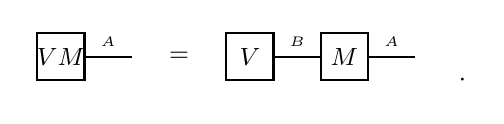
\begin{tikzpicture}[scale=0.3,thick] % , baseline = -3.5pt

\draw (-9,2)--(-7,2) node[midway,above] {\tiny $\catvariableof{A}$};
\draw (-11,1) rectangle (-9,3);
\node[anchor=center] (text) at (-10,2) {\small $VM$};

\node[anchor=center] (text) at (-5,2) {\small ${=}$};

\draw (3,2)--(5,2) node[midway,above] {\tiny $\catvariableof{A}$};
\draw (1,1) rectangle (3,3);
\node[anchor=center] (text) at (2,2) {\small $M$};
\draw (1,2)--(-1,2) node[midway,above] {\tiny $\catvariableof{B}$};
\draw (-1,1) rectangle (-3,3);
\node[anchor=center] (text) at (-2,2) {\small $V$};

\node[anchor=center] (text) at (7,1) {$\cdot$};


\end{tikzpicture}